\documentclass{article}

% NeurIPS 2026 template — comes bundled in the zip from:
% https://neurips.cc/Conferences/2026/CallForPapers
% Upload the zip to Overleaf as a new project, then paste this file over main.tex
\usepackage[preprint]{neurips_2026}

\usepackage[utf8]{inputenc}
\usepackage[T1]{fontenc}
\usepackage{hyperref}
\usepackage{url}
\usepackage{booktabs}
\usepackage{amsfonts}
\usepackage{amsmath}
\usepackage{amssymb}
\usepackage{nicefrac}
\usepackage{microtype}
\usepackage{xcolor}
\usepackage{graphicx}

\hypersetup{colorlinks=true, linkcolor=blue, citecolor=blue, urlcolor=blue}

\title{Can Free LLMs Serve as Practical Context Models for AIXI?\\
A Pilot Benchmark on Program-Generated Binary Sequences}

\author{%
  Ajinkya Awari \\
  SKNCOE, Pune, India \\
  \texttt{ajinkyaawari.skncoe.comp@gmail.com}
}

\begin{document}
\maketitle

% ----------------------------------------------------------------
\begin{abstract}
% ----------------------------------------------------------------

AIXI~\citep{hutter2000aixi} uses Solomonoff induction as its context model.
Solomonoff induction is incomputable, so a natural question arises: can modern
large language models (LLMs) fill that role in practice?
We introduce \textbf{SolomonoffBench}, a reproducible benchmark that probes
this question using 300 binary sequences generated by Turing machines (TMs)
with formally computed program lengths (24--60 bits) across four complexity
levels. As a pilot, we measure the \emph{gzip-normalized excess code length}
(\texttt{EL\_gzip}), the per-symbol gap between LLM cross-entropy and
incremental gzip conditional code length, for two free Qwen2.5 base models
run on a single Kaggle T4 GPU.
Neither model approaches the gzip baseline: Qwen2.5-3B averages
0.94~bits/sym above gzip (below the random ceiling of 1.0~bits/sym);
Qwen2.5-1.5B averages 1.06~bits/sym, failing to beat even random prediction.
More importantly, both models show near-flat \texttt{EL\_gzip} across all
four complexity levels ($\Delta \leq 0.068$~bits/sym), revealing that
incremental gzip is too coarse to detect algorithmic complexity gradients at
100-symbol windows.
This directly motivates a CTW-normalized Solomonoff Gap (SG) metric in v2.
Code and data: \url{https://github.com/ajinkya-awari/solomonoff-bench}.

\end{abstract}

% ----------------------------------------------------------------
\section{Introduction}
% ----------------------------------------------------------------

\citet{deletang2023language} showed that LLMs are competitive lossless
compressors on natural language and code, but their experiment holds
corpus \emph{type} fixed while varying content — it does not isolate
formally computed Kolmogorov complexity as a controlled variable.
The question we address is different: as the program length of the
generating Turing machine grows from 24 to 60 bits, does the gap between
LLM prediction and a compression baseline grow in step?
This K-conditioned design is motivated directly by AIXI
theory~\citep{hutter2000aixi,hutter2007universal}: if LLMs tracked
algorithmic complexity, they would be natural candidates to replace
Solomonoff induction~\citep{solomonoff1964formal} inside AIXI-like
agents~\citep{legg2007universal}.

Our pilot does not answer that question definitively — the gzip baseline
is too coarse for that — but it validates the measurement pipeline and
quantifies how far current free models are from even the gzip floor,
let alone from the theoretical Solomonoff bound.

\textbf{Contributions.}
\begin{itemize}
  \item \textbf{Benchmark design.}
        SolomonoffBench uses 300 TM-generated binary sequences with formally
        computed program lengths, providing a K-conditioned test bed for any
        sequence-prediction model.
  \item \textbf{Zero-cost pipeline.}
        Direct forward-pass logit scoring for HuggingFace base models on
        Kaggle T4 GPUs, with mandatory tokenizer validation and negative-delta
        logging — fully reproducible at zero compute cost.
  \item \textbf{Pilot findings.}
        Neither tested model beats gzip; only the 3B model beats random
        prediction. Both models are insensitive to the complexity gradient,
        establishing the need for a CTW-normalized baseline in v2.
\end{itemize}

% ----------------------------------------------------------------
\section{Background}
\label{sec:background}
% ----------------------------------------------------------------

\textbf{Kolmogorov complexity.}
The Kolmogorov complexity $K(x)$ of a binary string $x$ is the length of the
shortest program on a fixed universal Turing machine that produces~$x$~%
\citep{li2008vitanyi}.
Because it is upper-semicomputable, all practical estimates are proxies.
We use program bit length under a fixed TM encoding as a machine-specific
proxy $K_{\mathcal{M}}(x)$; we call this ``program bits'' throughout to avoid
overclaiming universality.

\textbf{Solomonoff induction and AIXI.}
Solomonoff induction~\citep{solomonoff1964formal} assigns probability
$\propto 2^{-K(x_{1:t})}$ to each prefix $x_{1:t}$, making it the
theoretically optimal sequence predictor.
AIXI~\citep{hutter2000aixi} couples Solomonoff induction with sequential
decision theory to define a universal intelligent agent.
Since Solomonoff induction is incomputable, practical AIXI implementations
need a tractable approximation.

\textbf{Context Tree Weighting (CTW).}
CTW~\citep{willems1995ctw} is the best known practical approximation to
Solomonoff induction for binary sequences.
It is parameter-free, converges to the optimal code length for
tree-structured sources, and achieves redundancy $O(\log n / n)$ per symbol.
In v2 we will use CTW to define the \emph{Solomonoff Gap}:
\begin{equation}
  \text{SG}(M, x) \;=\; H(M, x) - H_{\text{CTW}}(x)
  \quad \text{[bits per symbol]}
  \label{eq:sg}
\end{equation}
where $H(M, x)$ is the LLM's per-symbol cross-entropy.
$\text{SG} = 0$ means the model matches the best practical universal predictor;
$\text{SG} > 0$ quantifies the remaining gap.
\texttt{EL\_gzip} and SG are distinct metrics and are never plotted on a
common axis.

\textbf{Week~1 pilot metric (\texttt{EL\_gzip}).}
We substitute incremental gzip for CTW as a computationally minimal first
baseline:
\begin{equation}
  \texttt{EL\_gzip}(M, x) \;=\; H(M, x) - H_{\text{gzip}}^{\text{incr}}(x)
  \label{eq:elgzip}
\end{equation}
At 100-symbol windows, incremental gzip averages 0.036~bits/sym on
these ASCII binary strings (174 of 600 sequence-model pairs produce a
non-zero incremental cost; no negative deltas occur), so
\texttt{EL\_gzip} $\approx H(M, x)$ in practice.
The scale is: \texttt{EL\_gzip}~$= 0$ matches gzip;
\texttt{EL\_gzip}~$= 1.0$ matches a fair-coin random predictor;
\texttt{EL\_gzip}~$> 1.0$ is worse than random.

% ----------------------------------------------------------------
\section{SolomonoffBench}
\label{sec:bench}
% ----------------------------------------------------------------

\textbf{Sequence generation.}
We simulate a one-tape binary \emph{output transducer}: the symbol written at
each transition is appended to an output stream (not read from the tape).
Each TM runs for up to $10{,}000$ steps; machines that fail to emit
exactly 200 binary symbols are discarded.
Sequences are stored as ASCII strings of \texttt{"0"}/\texttt{"1"}
characters (one byte per symbol) to avoid packed-binary artefacts in gzip.

\textbf{Program bit encoding.}
For an $n$-state, 2-symbol TM, each transition rule requires
$2 + \lceil\log_2(n{+}1)\rceil$ bits (1~bit write symbol,
1~bit direction, $\lceil\log_2(n{+}1)\rceil$ bits next state),
giving $n \times 2 \times (2 + \lceil\log_2(n{+}1)\rceil)$ total program bits.

\textbf{Week~1 dataset.}
75 unique sequences are sampled per complexity level after within-level
deduplication of identical 200-symbol outputs, yielding 300 sequences total.
Table~\ref{tab:results} lists the four levels.
Transition tables, seeds, step counts, and discard rates are included in the
released dataset.

% ----------------------------------------------------------------
\section{Experimental Setup}
\label{sec:setup}
% ----------------------------------------------------------------

\textbf{Models.}
We evaluate \texttt{Qwen/Qwen2.5-3B} and \texttt{Qwen/Qwen2.5-1.5B}
\citep{qwen2025qwen25} on a single Kaggle T4 GPU (15~GB VRAM) at zero cost.
Both are free, ungated \emph{base} models.
Instruction-tuned variants assign near-zero mass to bare binary completion
tokens and fail the tokenizer validation gate; base models do not.

\textbf{Forward-pass scoring.}
We extract next-token log-probabilities via direct forward pass —
not \texttt{model.generate()} — at the final input token position:
\begin{equation}
  \hat{P}_M(b \mid x_{1:t})
  = \frac{\displaystyle\sum_{v \in V_b} e^{z_v}}
         {\displaystyle\sum_{w} e^{z_w}},
  \quad b \in \{0, 1\}
  \label{eq:prob}
\end{equation}
where $z$ are the last-position logits and $V_b$ is the set of token IDs
whose decoded string strips to~$b$.
The invalid-token mass $1 - \hat{P}_M(0) - \hat{P}_M(1)$ is logged
\emph{before} renormalization and archived in \texttt{benchmark\_log.jsonl};
all reported scores use renormalized probabilities.

\textbf{Prompt format.}
\begin{verbatim}
  Here is a binary sequence: 0 1 0 0 1 1 0 ...
  The next symbol is:
\end{verbatim}
The trailing space places the predicted bit at the next token position.
We score 100 consecutive positions per sequence given 100 symbols of context.

\textbf{Incremental gzip baseline.}
For context $c$ (100~chars) and prediction window $p$ (100~chars):
\begin{equation}
  H_{\text{gzip}}^{\text{incr}}(c, p)
  = \frac{8\,\bigl(\lvert\texttt{gzip}(c \,\|\, p)\rvert
                  - \lvert\texttt{gzip}(c)\rvert\bigr)}{|p|}
  \label{eq:gzip}
\end{equation}
Negative deltas (where adding the suffix \emph{shrinks} the archive)
are logged but never clamped; none occurred across 300 sequences.

\textbf{Tokenizer validation gate.}
Before any full run, $\hat{P}_M(0) + \hat{P}_M(1) \geq 0.01$ is verified
on five held-out toy sequences.
Both models clear this gate (valid binary mass: 65.4\%~for~3B,
63.5\%~for~1.5B).

% ----------------------------------------------------------------
\section{Results}
% ----------------------------------------------------------------

\begin{figure}[t]
  \centering
  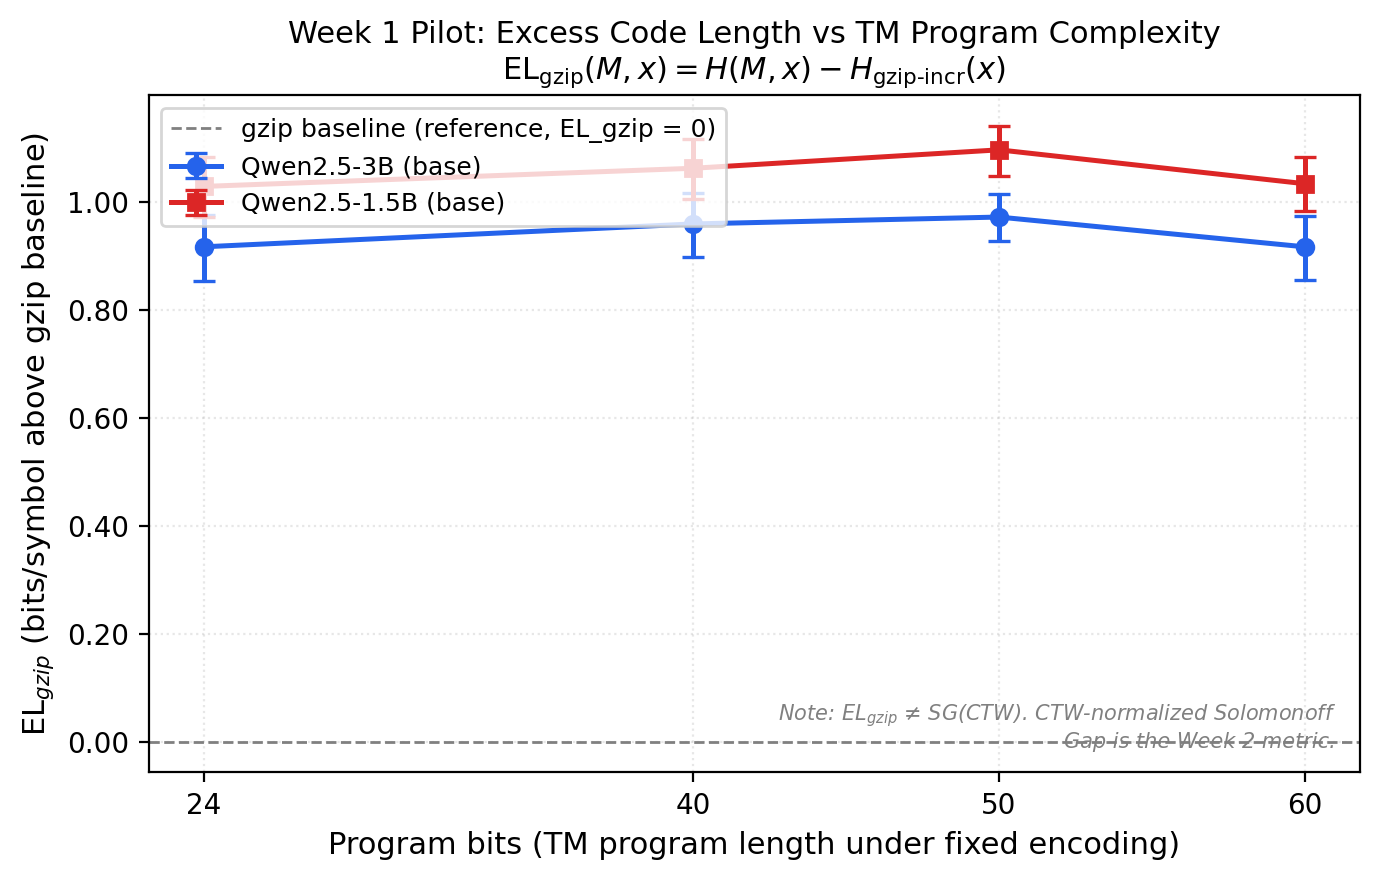
\includegraphics[width=0.85\linewidth]{figures/fig1_mvp_el_gzip.png}
  \caption{%
    \textbf{EL\_gzip vs.\ program bits — Week~1 pilot.}
    Mean gzip-normalized excess code length with 95\% bootstrap CI.
    The lower dashed line ($\texttt{EL\_gzip} = 0$) is the gzip baseline;
    the upper dashed line ($\texttt{EL\_gzip} = 1.0$) is the random-predictor
    ceiling.
    Qwen2.5-3B sits between the two baselines (better than random, worse than
    gzip); Qwen2.5-1.5B exceeds the random ceiling at all levels.
    The near-flat profiles ($\Delta \leq 0.068$~bits/sym across 24--60~program
    bits) show that incremental gzip is too coarse to discriminate complexity
    levels in this range, motivating the CTW-normalized SG in v2.%
  }
  \label{fig:main}
\end{figure}

\begin{table}[h]
\centering
\caption{%
  Week~1 pilot results: mean \texttt{EL\_gzip} $\pm$ std (bits/sym),
  75~sequences per level.
  Gzip baseline = 0.000 (reference); random ceiling = 1.000.
  Inv.\ mass: invalid-token fraction logged before renormalization.
  Negative gzip deltas: 0\,/\,300 for both models.%
}
\label{tab:results}
\vspace{4pt}
\small
\begin{tabular}{lcrrrrrr}
\toprule
Model & Params
  & L1 (24\,b) & L2 (40\,b)
  & L3 (50\,b) & L4 (60\,b) & Inv.\ mass \\
\midrule
Qwen2.5-3B   & 3.1B
  & $0.917{\pm}0.28$ & $0.959{\pm}0.27$
  & $0.972{\pm}0.19$ & $0.917{\pm}0.27$ & 34.3\% \\
Qwen2.5-1.5B & 1.5B
  & $1.028{\pm}0.24$ & $1.062{\pm}0.25$
  & $1.096{\pm}0.20$ & $1.034{\pm}0.23$ & 35.9\% \\
\midrule
gzip baseline  & ---
  & 0.000 & 0.000 & 0.000 & 0.000 & --- \\
random ceiling & ---
  & 1.000 & 1.000 & 1.000 & 1.000 & --- \\
\bottomrule
\end{tabular}
\end{table}

Figure~\ref{fig:main} and Table~\ref{tab:results} summarise the Week~1
results. Three findings stand out.

\textbf{Finding 1 — Both models fall short of gzip; only the larger beats random.}
Qwen2.5-3B produces \texttt{EL\_gzip} in the range 0.917--0.972~bits/sym:
above the gzip floor (0.000) but below the random ceiling (1.000), meaning
the 3B model at least extracts some predictive signal from the binary context.
Qwen2.5-1.5B scores 1.028--1.096~bits/sym, exceeding the random ceiling at
every level.
No tested model comes close to gzip compression performance at these
window sizes — a result that, within this two-model pilot using a weak
gzip baseline, suggests current free LLMs are poor practical substitutes
for even a simple compressor on algorithmically structured sequences.

The 1.5B result warrants a v2 recheck: exceedances of 0.028--0.096~bits/sym
above the random ceiling are small enough that non-uniform invalid-token
mass (35.9\% here) amplifying renormalization error cannot be ruled out
without a direct base-2 entropy cross-check against the raw logits.

\textbf{Finding 2 — Near-flat profiles reveal the baseline's inadequacy.}
The spread of mean \texttt{EL\_gzip} across the four complexity levels is
only 0.055~bits/sym (Qwen2.5-3B) and 0.068~bits/sym (Qwen2.5-1.5B).
Given that program lengths span 24--60~bits — a $2.5\times$ range — the
absence of a monotonic trend is striking.
The most likely explanation is not model insensitivity but baseline
insensitivity: incremental gzip on 100-character ASCII binary strings
trivially compresses most inputs to near-zero incremental cost, leaving
\texttt{EL\_gzip} dominated by $H(M, x)$ alone.
A baseline with per-symbol probability estimates (CTW) is needed to
separate the model's contribution from baseline noise.

\textbf{Finding 3 — Non-monotonic dip at Level~4.}
Both models show lower \texttt{EL\_gzip} at Level~4 (60~bits, 6-state TMs)
than at Level~3 (50~bits, 5-state TMs), returning approximately to Level~1
values.
We attribute this to the near-uniform-entropy character of 6-state TM
outputs: sequences that look like fair-coin draws give \emph{any} predictor
an easier cross-entropy target ($H(M, x)$ approaches 1.0~bit/sym).
We report this as a dataset property rather than a model behaviour claim.

\textbf{Tokenizer validity.}
Invalid-token mass of 34--36\% is expected for base models prompted in
natural language; all scores use renormalized binary probabilities.
The validation gate (binary mass $\geq 0.01$) passed on every model before
the full run.

% ----------------------------------------------------------------
\section{Discussion}
% ----------------------------------------------------------------

\textbf{What this means for AIXI.}
The most direct reading of Finding~1 is discouraging for AIXI-LLM hybrids:
two free base models cannot match even incremental gzip on program-generated
binary sequences.
A practical AIXI context model must outperform universal-coding baselines,
not merely approach a random predictor.
That said, the pilot covers only two models and uses a weak baseline; the
negative result is a lower bound, not a ceiling.
If CTW-normalized SG in v2 reveals that the gap shrinks at lower complexity
levels, it would suggest that LLMs are viable AIXI context models for simple
algorithmic inputs and degrade gracefully as complexity grows — a structured
failure mode more informative than a flat rejection.

\textbf{Why CTW is necessary.}
DEFLATE compression on 100-byte windows is near-perfect for short ASCII
binary strings: the algorithm finds run-length and Huffman codes that
reduce the incremental cost to a measured mean of 0.036~bits/sym
(Section~\ref{sec:background}) regardless of the sequence's
Kolmogorov complexity.
CTW~\citep{willems1995ctw} produces per-symbol probability estimates
with provable $O(\log n)$ redundancy, making it sensitive to the
complexity gradient that gzip misses entirely.
The flat profile in Figure~\ref{fig:main} is therefore not a null result —
it is the empirical justification for the upgrade.

\textbf{Limitations.}
\begin{itemize}
  \item $K_{\mathcal{M}}(x)$ is machine-specific; universality claims
        require a bounded shorter-TM check, especially at low state counts.
  \item Only two model sizes; at least four data points are needed before
        any claim about model-size scaling.
  \item Invalid-token mass of~$\sim$35\% means roughly one third of model
        capacity is wasted on non-binary outputs.
  \item CTW converges to the optimal code length for tree-structured sources,
        not for all computable measures; SG therefore lower-bounds the true
        Solomonoff gap.
\end{itemize}

% ----------------------------------------------------------------
\section{Conclusion}
% ----------------------------------------------------------------

SolomonoffBench provides a reproducible K-conditioned test bed for measuring
how far LLMs fall from theoretical prediction optimality on algorithmically
structured binary sequences.
The Week~1 pilot establishes two things: neither tested free model beats
incremental gzip, and neither model's excess loss grows with program complexity
in the 24--60~bit range.
Both findings point to the same conclusion — a CTW-normalized Solomonoff Gap
metric is required to resolve whether LLMs can serve as practical AIXI context
models.
All code, data, and benchmark figures are released at
\url{https://github.com/ajinkya-awari/solomonoff-bench}.

\begin{ack}
Compute provided by Kaggle (free T4 GPU tier).
Models accessed via HuggingFace Transformers~\citep{wolf2020transformers}.
Writing assistance provided by Claude (Anthropic, 2026).
No external funding.
\end{ack}

\bibliographystyle{plainnat}
\bibliography{references}

\end{document}
